
Порождающие модели современное и быстро развивающие направление работы с данными.

Ключевыми достижениями в дисципилине были \begin{enumerate}
    \item порождающие грамматики \cite{chomsky2002syntactic}
    \item графические вероятностные модели \cite{pearl1988probabilistic}
    \item состязательные порождающие модели \cite{goodfellow2020generative}
    \item диффузионные порождающие модели \cite{song2020score}
\end{enumerate}

Порождающие модели задают совместное распределение наблюдаемого объекта $x$ и его черт $y$ -  $p(x,y)$. В этом заключается 
ключевое различие между порождающими и дискриминирующими моделями $p(y|x)$ \ref{discr_vs_gen}.

\begin{figure}[h]
    \centering
    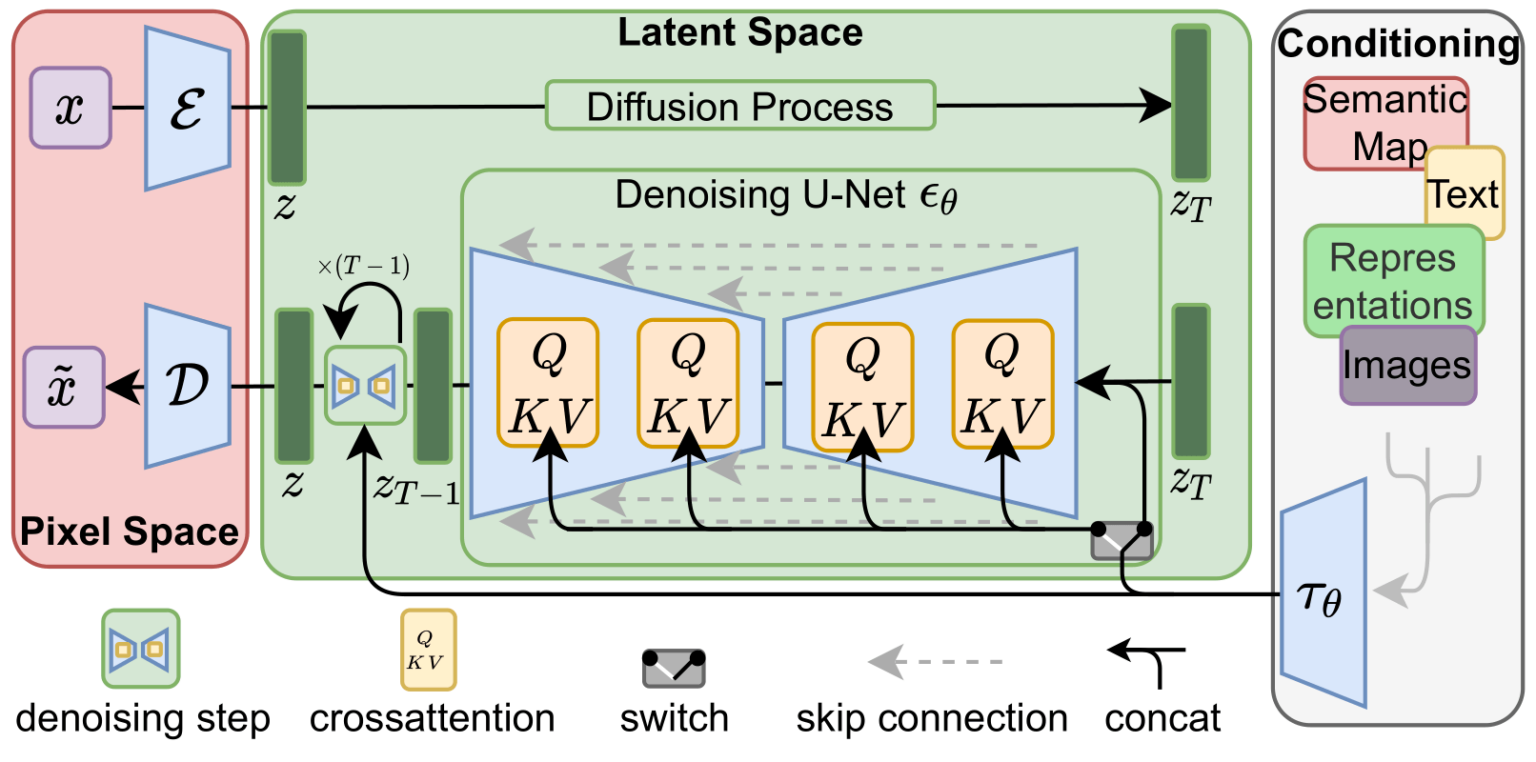
\includegraphics[width=0.5\textwidth]{assets/ml/generation/stable_diffusion.png}
    \caption{Генеративные отличаются}
    \label{discr_vs_gen}
\end{figure}


Порождающие модели, используют параметрические модели $p_\theta$ для аппроксимации истинных функций распределений. Таким образом, аппроксиматором может выступить
древо или нейросеть.

\textit{Определение} $f$-дивергенцией называется выпуклая функция, удовлетворяющая равенству $f(1)=0$/

$$
    D_f{\pi \parallel \rho} = \mathrm E_{\rho(x)} f\left(\frac{\pi(x)}{\rho(x)}\right)
$$

Семейство $f$-дивергенций включает функции \begin{enumerate}
    \item Кульбака-Лейбнера $f(u)=u logu $
\end{enumerate}


Нижней вариационной оценкой называется техника максимизации подпирающей границы параметрического распределения $p(\mathbf{x},\mathbf{z})$ вторым $q(\mathbf{x},\mathbf{z})$,
где переменная $\mathbf{z}$ называется скрытой . В аналитической форме нижняя граница записывается как 
$$
    \mathcal{L}(\phi,\theta;x) = \mathbb{E}_{z \sim q_\phi(z|x)} \left[\ln \frac{p_{\theta}(x,z)}{q_{\phi}(z|x)}\right],
$$

Ключевым свойством полученной оценки является выражение:
$$
    \ln p_\theta(x) \le \mathcal{L}(\phi,\theta;x)
$$
полученное из частного случая неравенстов Йенсена.


\textit{Определение} \textbf{EM-алгоритм} - алгоритм для нахождения оценок
максимального правдоподобия параметров  вероятностных моделей с скрытыми переменными $\theta$.

Алгоритм состоит из двух шагов. \begin{itemize}
    \item E(xpectation) шага $q^{(t)} = $. Шаг 
    обновляет распределение при фиксированных параметрах
    \item M(maximization) $\Theta$ является значением, 
    максимизирующим на шаге $M$ условное матожидание $E$ логарифма правдоподобия при данных значениях наблюдаемых переменных и предыдущем значении параметров.  
\end{itemize}
